\documentclass[10pt]{article}

\usepackage[margin=1in]{geometry}
\usepackage{graphicx}
\usepackage{booktabs}
\usepackage{amsmath}
\usepackage{amssymb}
\usepackage{hyperref}
\usepackage{xcolor}

\title{Quality-Calibrated Localization-Guided VLM Reasoning for Industrial Anomaly Recognition}
\author{Anonymous Authors}
\date{}

\begin{document}
\maketitle

\begin{abstract}
Industrial anomaly recognition with general-purpose vision-language models remains unreliable when defects are small, localized, and visually subtle.
We propose Quality-Calibrated QCR, a localization-guided VLM reasoning framework that converts detector localization evidence into candidate-level visual-language evidence and calibrates crop-level VLM anomaly scores using candidate quality.
The method treats candidate quality as the main reliability mechanism and uses detector-VLM consistency only as a conservative adaptive refinement.
Experiments with detector, VLM, and external anomaly baselines show that localization-guided VLM evidence complements detector scores.
Ablations further show that quality calibration provides the main gain over naive detector-crop fusion, while adaptive consistency yields only a small refinement and fixed consistency should remain diagnostic.
Failure and boundary analyses clarify when quality calibration helps, when it fails, and why broad claims about segmentation or manufacturing-cause reasoning are unsupported.
\end{abstract}

\section{Introduction}

Industrial anomalies often occupy small localized regions and may not dominate global image semantics~\cite{Bergmann2019MVTecAD,Zou2022VisA}.
This makes direct full-image VLM reasoning unreliable for industrial inspection.
A detector can provide localization evidence, while a VLM can provide visual-language abnormality evidence; however, naive fusion does not model whether the localized crop is reliable.
We address this gap by calibrating crop-level VLM scores with candidate quality derived from localization evidence.

Our method, \emph{Quality-Calibrated QCR}, uses detector localization to generate candidate crops, obtains crop-level VLM anomaly evidence, and modulates that evidence using candidate quality.
We also study detector-VLM consistency, but robustness analysis shows that fixed consistency is not reliable enough to be the final method.
Thus, consistency is retained only as a small adaptive refinement.

Our contributions are:
\begin{itemize}
    \item We formulate industrial anomaly recognition as localization-guided VLM evidence reasoning.
    \item We propose candidate-quality calibration as the main reliability mechanism for crop-level VLM evidence.
    \item We analyze fixed and adaptive detector-VLM consistency and show why consistency must be treated conservatively.
    \item We provide strong baseline comparisons, ablations, boundary analysis, and fixed-budget sensitivity checks with explicit claim restrictions.
\end{itemize}

\section{Related Work}

\paragraph{Industrial anomaly detection.}
PatchCore~\cite{Roth2022PatchCore}, FastFlow-style detectors~\cite{Yu2021FastFlow}, and EfficientAD~\cite{Batzner2024EfficientAD} provide strong anomaly detection and localization evidence.
Our method does not replace these detectors; it uses localization evidence to produce candidate-level VLM evidence.

\paragraph{Vision-language anomaly detection.}
CLIP~\cite{Radford2021CLIP}-based anomaly methods such as WinCLIP~\cite{Jeong2023WinCLIP} and AnomalyCLIP~\cite{Zhou2024AnomalyCLIP} show the value of language-supervised representations.
Our work is narrower: it studies how detector-guided crop evidence should be calibrated before being trusted by a VLM-based anomaly scorer.

\paragraph{Reliability calibration.}
Naive score fusion assumes detector and VLM scores are equally reliable.
We show that candidate quality is the stable calibration signal, whereas fixed consistency is not robust enough to be the final method.

\section{Method}

Given image $x$, a detector produces localization evidence $A$ and normalized anomaly score $D$.
Candidate crops $C=\{c_i\}$ are generated from $A$.
The VLM scores each crop and the crop-level scores are aggregated into $M$.
Candidate quality $Q$ measures the reliability of the localized crop evidence.

The naive detector-crop fusion baseline is:
\begin{equation}
S_{\mathrm{naive}} = 0.5D + 0.5M.
\end{equation}

Quality-Calibrated QCR modulates the VLM contribution by candidate quality:
\begin{equation}
S_{\mathrm{quality}} = 0.5D + 0.5M(0.5 + 0.5Q).
\end{equation}

A diagnostic fixed Q+C variant is:
\begin{equation}
S_{\mathrm{fixed}} = 0.4D + 0.4M + 0.1Q + 0.1K,
\end{equation}
where $K$ is detector-VLM high-high consistency.
This variant is diagnostic only because fixed consistency is not robust across protocols.

The adaptive refinement uses a conservative gate:
\begin{equation}
g = QK(1-|D-M|)\min(D,M),
\end{equation}
\begin{equation}
S_{\mathrm{adaptive}} = S_{\mathrm{quality}} + 0.05g.
\end{equation}

The main method is $S_{\mathrm{quality}}$.
The adaptive variant is reported as a refinement, not as the main performance source.

\begin{figure}[t]
\centering
\fbox{
\begin{minipage}{0.92\linewidth}
\centering
\vspace{0.8em}
\textbf{Figure 1 placeholder.}\\
Detector localization $\rightarrow$ candidate crops $\rightarrow$ crop VLM score $\rightarrow$ candidate quality calibration $\rightarrow$ adaptive refinement.\\
The SVG source is stored at \texttt{figures/figure1\_framework\_schematic.svg}.
\vspace{0.8em}
\end{minipage}
}
\caption{Overview of Quality-Calibrated QCR. Candidate quality is the main method core; adaptive consistency is a conservative refinement; fixed Q+C is diagnostic only.}
\label{fig:framework}
\end{figure}

\section{Experiments}

We evaluate two complementary views.
The system-level view compares VLM baselines, detector baselines, and localization-guided fusion, using VisA-style industrial anomaly evaluation context~\cite{Zou2022VisA}.
The QCR view isolates detector-only scoring, crop VLM scoring, naive fusion, quality calibration, fixed Q+C, and adaptive refinement under the QCR primary protocol.
Image AUROC is the main metric; pixel metrics are auxiliary only.

\section{Main Results}

Full-image VLM obtains mean AUROC 0.6459, while context-aware VLM obtains 0.7101.
PatchCore~\cite{Roth2022PatchCore} obtains 0.7853 and EfficientAD-30 fixed-budget~\cite{Batzner2024EfficientAD} obtains 0.7604.
The fair LOCO fusion reaches 0.8210, improving over PatchCore by +0.0356 and over EfficientAD-30 by +0.0606.
The same-set result 0.8453 is reported only as an upper-bound diagnostic.

\begin{table}[t]
\centering
\caption{System-level strong baseline comparison.}
\label{tab:system_baselines}
\resizebox{\linewidth}{!}{%
\begin{tabular}{@{}llll@{}}
\toprule
Method & Mean AUROC & Role & Protocol \\
\midrule
PatchCore + context VLM, same-set & 0.8453 & upper\_bound\_diagnostic\_only & mean\_summary \\
PatchCore + context VLM, LOCO & 0.8210 & primary\_fair\_system\_result & mean\_summary \\
PatchCore & 0.7853 & classic\_detector\_baseline & mean\_summary \\
EfficientAD-30 fixed-budget & 0.7604 & modern\_detector\_fixed\_budget\_baseline & mean\_summary \\
context-aware VLM & 0.7101 & vlm\_baseline & mean\_summary \\
full-image VLM & 0.6459 & vlm\_baseline & mean\_summary \\
WinCLIP fixed protocol & 0.6138 & external\_vlm\_anomaly\_baseline & mean\_summary \\
\bottomrule
\end{tabular}%
}
\vspace{2pt}
\footnotesize{\emph{Note.} LOCO is the fair system-level result. Same-set is an upper-bound diagnostic only.}
\end{table}


\section{Ablation Study}

Under the QCR primary protocol, naive detector-crop fusion obtains mean AUROC 0.9652.
Quality-Calibrated QCR obtains 0.9748, a gain of +0.0096.
The adaptive refinement obtains 0.9752, improving over naive fusion by +0.0100 but over the quality core by only +0.0004.
Therefore, the main effective component is candidate quality calibration, not adaptive consistency.

\begin{table}[t]
\centering
\caption{QCR primary-protocol ablation.}
\label{tab:qcr_ablation}
\resizebox{\linewidth}{!}{%
\begin{tabular}{@{}llllll@{}}
\toprule
ID & Method & FastFlow & PatchCore & Mean AUROC & Role \\
\midrule
V0 & Detector only & 0.8955 & 0.9131 & 0.9043 & anchor\_baseline \\
V2 & Crop VLM only & 0.9269 & 0.8846 & 0.9057 & vlm\_crop\_baseline \\
V3 & Naive detector-crop fusion & 0.9688 & 0.9616 & 0.9652 & naive\_fusion\_baseline \\
V4 & Quality-Calibrated QCR & 0.9778 & 0.9718 & 0.9748 & main\_effective\_method\_core \\
V5 & Fixed Q+C fusion & 0.9842 & 0.9740 & 0.9791 & diagnostic\_not\_final \\
V6 & Quality-Calibrated QCR + adaptive consistency refinement & 0.9783 & 0.9722 & 0.9752 & final\_refinement\_variant \\
\bottomrule
\end{tabular}%
}
\vspace{2pt}
\footnotesize{\emph{Note.} Quality-Calibrated QCR is the main method core. Fixed Q+C is diagnostic only.}
\end{table}


\section{Failure and Boundary Analysis}

Boundary analysis shows that quality calibration is useful but not universal.
It can help by boosting true localized anomalies or suppressing normal false positives, but it can also fail when candidate quality is misleading or detector-VLM evidence disagrees.
Fixed Q+C can peak in some cases but is not robust enough to be final.

\begin{figure}[t]
\centering
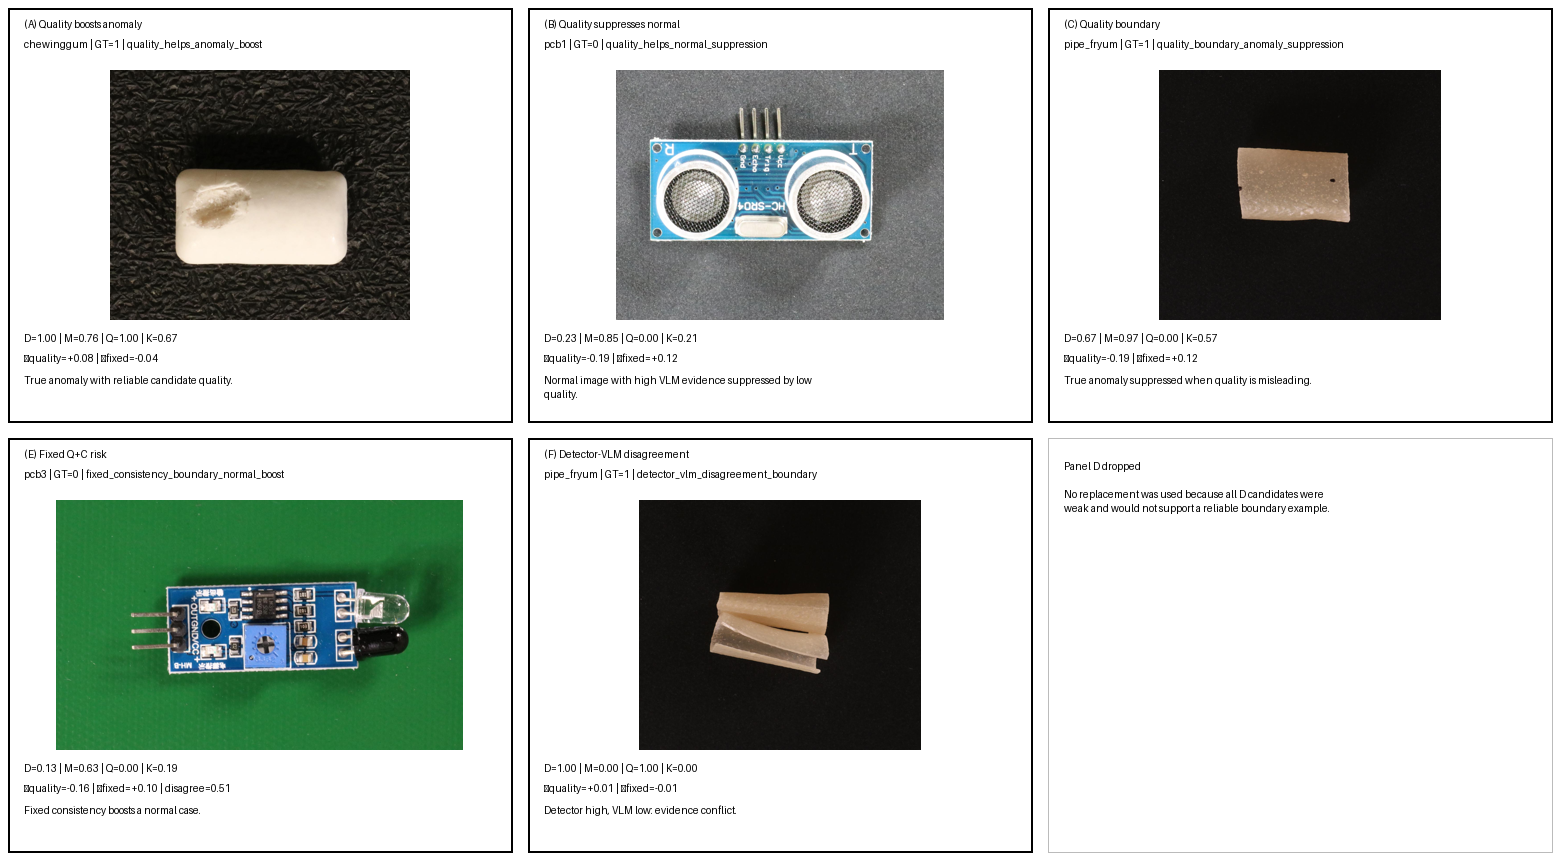
\includegraphics[width=\linewidth]{figures/figure2_boundary_cases_montage.png}
\caption{Representative boundary cases for quality-calibrated localization-guided VLM reasoning. Quality calibration can boost true anomaly evidence and suppress normal false positives, but it can also fail when candidate quality is misleading. Fixed Q+C can over-boost normal evidence, and detector-VLM disagreement remains a boundary case. These examples illustrate method boundaries rather than universal behavior.}
\label{fig:boundary_cases}
\end{figure}

\begin{table}[t]
\centering
\caption{Boundary and robustness summary.}
\label{tab:boundary_summary}
\resizebox{\linewidth}{!}{%
\begin{tabular}{@{}llllll@{}}
\toprule
Comparison & Mean delta & Wins & Min & Max & Interpretation \\
\midrule
Quality-Calibrated QCR - Naive & +0.0119 & 13/24 & -0.0132 & +0.0908 & quality calibration \\
Adaptive - Quality-Calibrated QCR & +0.0003 & 14/24 & +0.0000 & +0.0014 & adaptive refinement \\
Fixed Q+C - Quality-Calibrated QCR & +0.0027 & 18/24 & -0.0506 & +0.0202 & diagnostic fixed consistency \\
Adaptive - Fixed Q+C & -0.0024 & 3/24 & -0.0189 & +0.0508 & robustness tradeoff \\
\bottomrule
\end{tabular}%
}
\vspace{2pt}
\footnotesize{\emph{Note.} Per-category deltas show quality calibration is useful but not universal; adaptive consistency is only a refinement.}
\end{table}


\section{EfficientAD Budget Sensitivity}

A 100-epoch EfficientAD sensitivity check on fruit_jelly gives image-AUROC delta -0.0167 relative to EfficientAD-30.
This does not indicate severe image-level underestimation of EfficientAD-30, but EfficientAD remains a fixed-budget baseline and should not be described as full EfficientAD defeat.

\begin{table}[t]
\centering
\caption{EfficientAD-100 fruit\_jelly sensitivity.}
\label{tab:efficientad_sensitivity}
\resizebox{\linewidth}{!}{%
\begin{tabular}{@{}llll@{}}
\toprule
Metric & EfficientAD-30 & EfficientAD-100 & Delta \\
\midrule
image\_AUROC & 0.8433 & 0.8267 & -0.0167 \\
image\_F1Score & 0.8571 & 0.8438 & -0.0134 \\
pixel\_AUROC & 0.7894 & 0.8424 & +0.0531 \\
pixel\_F1Score & 0.5395 & 0.5561 & +0.0166 \\
\bottomrule
\end{tabular}%
}
\vspace{2pt}
\footnotesize{\emph{Note.} This is a defensive fixed-budget sensitivity check, not a full EfficientAD sweep.}
\end{table}


\section{Limitations}

The method is image-level anomaly recognition and candidate-level VLM evidence calibration.
It does not claim pixel-level segmentation SOTA, manufacturing-cause reasoning, or full anomaly understanding.
EfficientAD is fixed-budget, AnomalyCLIP~\cite{Zhou2024AnomalyCLIP} is not experimentally included, and adaptive consistency has only a small gain over quality-only.

\section{Conclusion}

Quality-Calibrated QCR provides a reliability-calibrated bridge between industrial anomaly localization and VLM anomaly evidence.
Candidate quality is the main effective component, while adaptive consistency is a conservative refinement.
The evidence supports a cautious but coherent claim: localization-guided VLM anomaly recognition becomes more reliable when crop-level evidence is calibrated by candidate quality.

\bibliographystyle{plain}
\bibliography{references}

\end{document}
